\documentclass[12pt]{article}

\usepackage[
  margin=2cm,
  top=2cm,
  bottom=2cm
]{geometry}
\usepackage[utf8]{inputenc}
\usepackage[T1]{fontenc}
\usepackage[italian]{babel}

\usepackage{amsmath,amssymb,amsfonts}
\usepackage{graphicx}
\graphicspath{{../source/figures/}}
\usepackage{subcaption}
\usepackage{float}
\usepackage{fancyhdr}
\usepackage[nottoc,notlot,notlof]{tocbibind}

\usepackage{microtype} 

\title{Modello di Ising}
\author{Pivi Riccardo}
\date{Marzo 2026}

\begin{document}
\maketitle

\tableofcontents
\newpage

\section{Introduzione}
Per gran parte della storia della scienza moderna, il riduzionismo ha rappresentato la bussola metodologica predominante: 
l'idea che, per comprendere un sistema, sia sufficiente scomporlo nelle sue parti costituenti e studiarne le leggi fondamentali. Tuttavia,
nel 1972, il Premio Nobel Philip Anderson pubblicò su Science un articolo intitolato "More is Different" \cite{anderson}, 
scardinando questa visione.

Anderson sosteneva che la capacità di ridurre tutto a semplici leggi fondamentali non implica 
la capacità di ricostruire l'universo a partire da esse. Al crescere della complessità e del numero 
di componenti di un sistema, appaiono proprietà totalmente nuove, non deducibili in modo banale dalle 
leggi che governano i singoli elementi. Questo fenomeno è noto come comportamento emergente. I comportamenti emergenti sono proprietà macroscopiche 
di un sistema di cui i singoli componenti non sono portatori. Le proprietà macroscopiche 
non sono deducibili dalle leggi dei singoli, ma emergono dunque dall'interazione di molti elementi.

Un esempio paradigmatico per comprendere il concetto di emergenza è il modello di Ising. Esso descrive un sistema di spin interagenti su 
un reticolo. Ogni spin può assumere due stati, rappresentati da +1 (spin up) e -1 (spin down), e interagisce con i suoi vicini più prossimi.
Il modello di Ising è stato originariamente proposto per studiare il comportamento magnetico dei materiali ferromagnetici, in particolare di studiarne la transizione 
di fase tra uno stato disordinato ad alta temperatura e uno stato ordinato a bassa temperatura. La transizione di fase è un fenomeno emergente: essa non è infatti riconducibile alle proprietà del singolo spin —
il quale non possiede intrinsecamente una temperatura critica o una fase —
ma scaturisce esclusivamente dalla interazione collettive. Sotto la temperatura critica il sistema "sceglie" collettivamente 
una direzione preferenziale di orientazione, trasformando un insieme di interazioni 
locali in un ordine macroscopico manifestato dalla magnetizzazione spontanea.

L’obiettivo di questo lavoro è analizzare la transizione di fase nel modello di Ising attraverso tre prospettive complementari. In primo luogo,
verrà presentata la teoria di campo medio, che fornisce una descrizione analitica approssimata del fenomeno e consente di stimare la temperatura critica.
Successivamente, si studierà il modello tramite simulazioni numeriche Monte Carlo (MC) basate sull’algoritmo di Metropolis,
analizzando grandezze termodinamiche quali energia ($E$), magnetizzazione media ($m$), suscettibilità ($\chi$) e capacità termica ($C_v$)
al variare della temperatura. Inoltrè è stata stimata la temperatura crtica ($T_C$).
Infine, verrà applicata la Principal Component Analysis (PCA) alle configurazioni generate con MC, 
osservando come l'approccio con strumenti di machine learning non supervisionato 
abbia le potenzialità di scoprire transizioni di fase e di riconoscere il parametro d'ordine esclusivamente dalle caratteristiche dei dati.

\section{Il Modello di Ising}

\subsection{Storia}
Il modello di Ising è un modello matematico utilizzato in fisica statistica per descrivere il comportamento di sistemi magnetici. 
Fu introdotto ideato da Wilhelm Lenz nel 1920, che lo propose al suo studente di dottorato Ernst Ising come problema da risolvere. 
Ising nel 1925 pubblica la soluzione del modello in una dimensione \cite{ising1925}, solo nel 1944 Onsager 
pubblicherà la soluzione per il caso bidimensionale. 
Il modello rappresenta un sistema di spin su una griglia, dove ogni spin può assumere due stati:
 +1 (spin up) o -1 (spin down). Gli spin sono fra loro interagenti e possono essere influenzati da un campo magnetico esterno.
L'allinemento degli spin in una direzione specifica può portare a un comportamento collettivo 
che si manifesta come magnetizzazione. Il modello di Ising è stato ampiamente studiato per comprendere 
le transizioni di fase e il comportamento critico nei sistemi magnetici, ed è diventato un punto
di riferimento fondamentale nella fisica statistica. 
Inoltre il modello ha avuto successo anche in altri campi del sapere come le reti neurali (reti di Hopfield), biofisica e sociologia(modelli di opinione),
dimostrando la sua versatilità e importanza come strumento di modellizzazione in diverse discipline scientifiche.

\subsection{Definizione del Modello}
Per gli scopi di questo lavoro, ci concentreremo sul modello di Ising bidimensionale su un reticolo quadrato,
anche se il modello può essere definito in qualsiasi dimensione e su diversi tipi di reticoli.
Consideriamo un reticolo con $N$ siti, dove ogni sito $i$ è occupato da uno spin $s_i$ che può assumere i valori +1 o -1.
L'energia totale del sistema è data dalla seguente espressione:
\begin{equation}
E = -J \sum_{\langle i,j \rangle} s_i s_j - h \sum_{i} s_i  
\end{equation}

Il primo termine rappresenta l’interazione tra coppie di spin adiacenti: dove  $\langle i,j \rangle$ indica che la somma è effettuata sui siti adiacenti del reticolo ovvero sui vicini più prossimi. 
Il parametro $J$ è la costante di accoppiamento:

\begin{itemize}
\item Se $J > 0$, l’interazione è ferromagnetica e favorisce l’allineamento degli spin.
\item Se $J < 0$, l’interazione è antiferromagnetica.
\end{itemize}

Infatti per $J>0$ l'energia è minima quando gli spin sono allineati (tutti +1 o tutti -1), mentre per $J<0$ l'energia è minima quando gli spin sono anti-allineati (ad esempio, in un reticolo quadrato, ogni spin è circondato da spin di segno opposto).

Nel presente lavoro si considera il caso ferromagnetico ($J>0$) e campo esterno nullo ($h=0$), così che l’Hamiltoniana si riduce a:

\[
E = -J \sum_{\langle i,j \rangle} s_i s_j.
\]

L’equilibrio termodinamico del sistema è descritto dalla distribuzione di Boltzmann:

\[
P(\{s_i\}) = \frac{1}{Z} e^{-\beta H},
\]

dove $\beta = 1/(k_B T)$ e $Z$ è la funzione di partizione:

\begin{equation}
Z = \sum_{\{s_i\}} e^{-\beta E(\{s_i\})}    
\end{equation}

Dal punto di vista fisico, a basse temperature l’energia domina e il sistema tende ad assumere configurazioni ordinate con spin allineati. Ad alte temperature, invece, le fluttuazioni termiche prevalgono e il sistema si trova in uno stato disordinato.

In due dimensioni e campo nullo, il modello presenta una transizione di fase a una temperatura critica finita $T_c$, che separa una fase ferromagnetica (magnetizzazione spontanea non nulla) da una fase paramagnetica (magnetizzazione nulla).


\section{Teoria di campo medio e soluzione esatta}

\subsection{Teoria di campo medio}
La funzione di partizione del modello di Ising nel caso in cui il campo magnetico esterno sia assente ($h=0$) è:
\begin{equation}
Z = \sum_{\{s_i\}} e^{-\beta E(\{s_i\})} = \sum_{\{s_i\}} e^{\beta J \sum_{\langle i,j \rangle} s_i s_j}
\end{equation}

Dove $\beta = \frac{1}{k_B T}$ è l'inverso della temperatura. 
Calcolata la funzione di partizione possiamo ottenere tutte le proprietà del sistema attraverso l'energia libera $F$:

\begin{equation}
F = -k_B T \ ln Z
\end{equation}

La teoria di campo medio ci permette di calcolare un'approssimazione della funzione di partizione, 
assumendo che ogni spin sia influenzato da un campo magnetico medio generato dagli altri spin \cite{stanford_sml_susskind}.
In $d$ dimensioni ogni spin ha $z = 2 \ d $ vicini, l'energia di un singolo spin è data da:
\begin{equation}
E_i = -J s_i \sum_{j=1}^z s_j
\end{equation}
Considerando che ogni spin può essere $+1$ o $-1$, possiamo sostituire la somma con una media, ottenendo:
\begin{equation}
E_i = -J s_i z m
\end{equation}
Dove $m$ è la magnetizzazione media del sistema, definita come:
\begin{equation}
m = \langle s_i \rangle 
\end{equation}
La funzione di partizione diventa per un unico spin:
\begin{equation}
    Z = \sum_{s_i} e^{\beta J z m s_i} = e^{\beta J z m} + e^{-\beta J z m} = 2 \cosh(\beta J z m)
\end{equation}
L'energia media:
\begin{equation}
    \langle E \rangle= - \frac{1}{Z} \ \frac{\partial Z}{\partial \beta} = - J z m \tanh(\beta J z m)
\end{equation}
Confrontandola questa espressione con l'espressione precedente dell'energia otteniamo l'equazione:
\begin{equation}
    m = \langle s_i \rangle = \tanh(\beta J z m)
\end{equation}
Questa è una equazione trascendentale, che possiamo risolvere numericamente\cite{essential_statistical_physics}.

\begin{figure}[H]
    \centering
    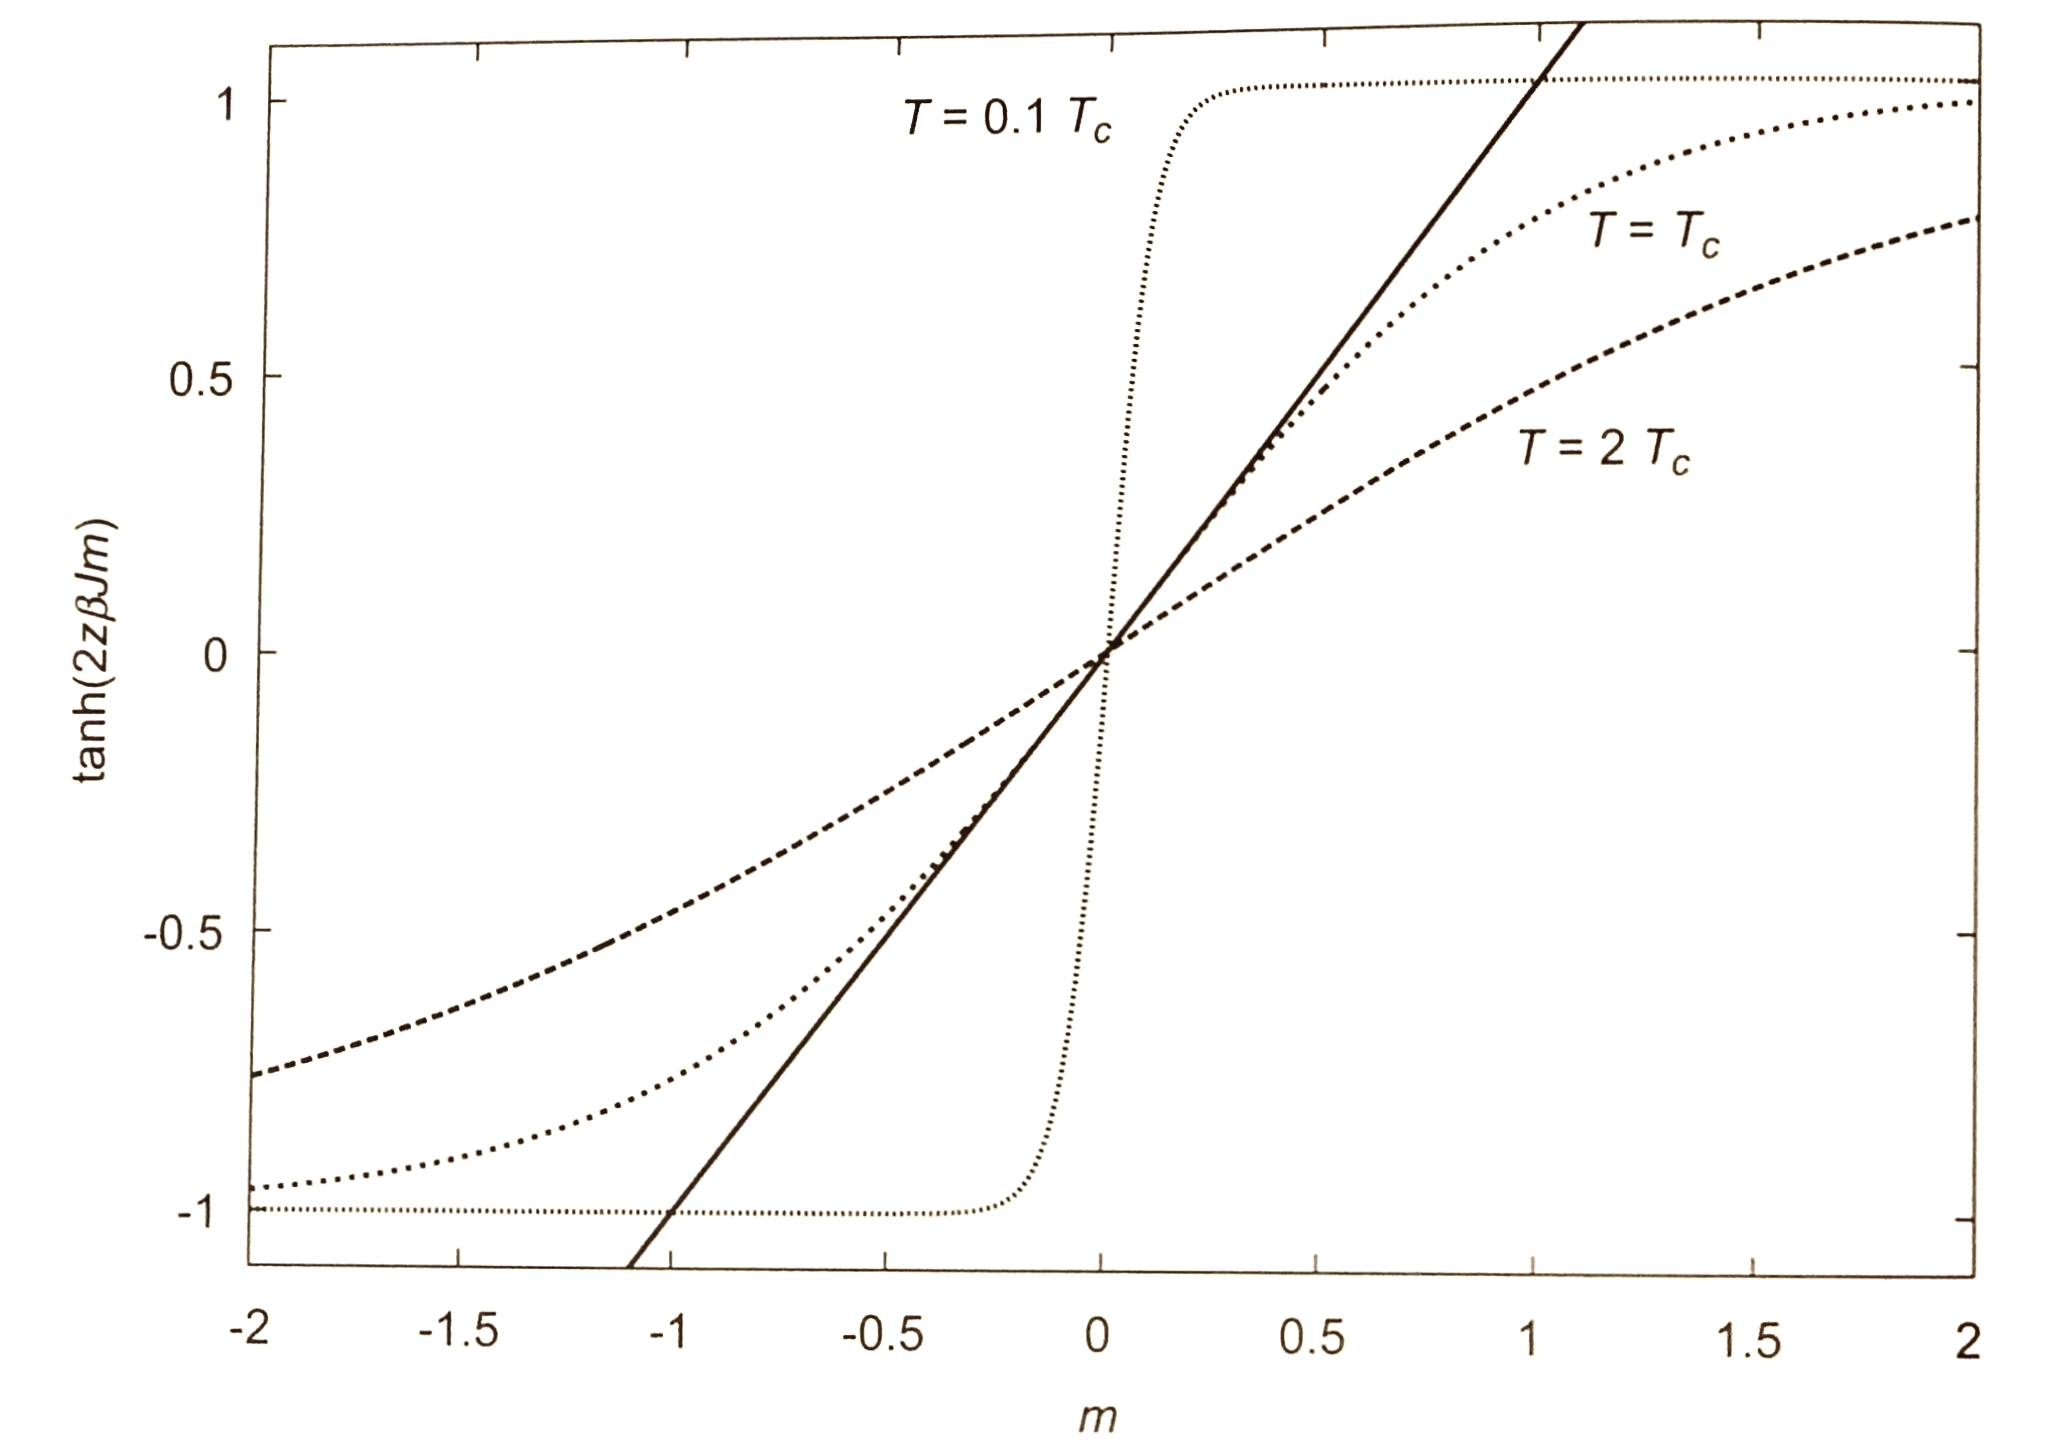
\includegraphics[width=0.6\textwidth]{kennett_trascendente.jpg}
    \caption{Soluzione numerica dell'equazione.}
    \label{fig:kennett_trascendente}
\end{figure}

L'equazione ha un unica soluzione per $z \beta J < 1$, mentre per $z \beta J > 1$ ne ha due; 
ovvero il sistema per temperature alte il sistema è in uno stato disordinato con magnetizzazione nulla, mentre per temperature basse il sistema è in uno stato ordinato con magnetizzazione diversa da zero.
In questo modo è possibile ottenere la temperatura critica stimata dalla teoria di campo medio imponendo che $z \beta J = 1$, da cui otteniamo:
\begin{equation}
    T_c = \frac{z J}{k_b}
\end{equation}

\subsection{Risultati della soluzione esatta}
La soluzione esatta del modello di Insing nel caso bidimensionale con $h=0$ è stata ottenuta per la prima volta da Lars Onsager nel 1944.
Onsager riusci a determinare la temperatura critica $T_c$ alla quale avviene la transizione di fase, e a calcolare esattamente la funzione di partizione e le proprietà termodinamiche del sistema.
La temperatura critica è data da:
\begin{equation}
    T_c = \frac{2J}{k_B \ln(1 + \sqrt{2})} \approx 2.269 J/k_B
\end{equation}
La quale è inferiore alla temperatura critica prevista dalla teoria di campo medio, la quale per il caso bidimensionale è $T_c^{MF} = 4J/k_B$. 
Il motivo della sovrastima è 

\section{Metodo Monte Carlo}

Lo studio del modello di Ising mediante simulazioni numeriche si basa su tecniche di campionamento stocastico. 
L’obiettivo è generare configurazioni di spin distribuite secondo la distribuzione di Boltzmann. Poiché il numero totale di configurazioni cresce come $2^N$, un campionamento esaustivo è impraticabile per sistemi macroscopici. 
Si utilizza quindi il metodo Monte Carlo con algoritmo di Metropolis per costruire una catena di Markov che converga alla distribuzione canonica.

\subsection{Algoritmo di Metropolis}

L’algoritmo di Metropolis permette di generare una sequenza di configurazioni $\{C_0, C_1, C_2, \ldots\}$ tale che,
dopo un numero sufficiente di passi,
la distribuzione delle configurazioni sia quella desiderata, ovvero la distribuzione di Boltzmann.
L’algoritmo procede come segue:

\begin{enumerate}
    \item Si sceglie casualmente un sito $i$ del reticolo.
    \item Si propone il flip dello spin $s_i \rightarrow -s_i$.
    \item Si calcola la variazione di energia $\Delta E$ associata al flip.
    \item Il flip viene accettato con probabilità
    \begin{equation}
    P_{\text{acc}} = \min\left(1, e^{-\beta \Delta E}\right).
    \end{equation}
\end{enumerate}

Questo criterio garantisce il rispetto della condizione di bilancio dettagliato:

\begin{equation}
\frac{P(C \rightarrow C')}{P(C' \rightarrow C)} = e^{-\beta (E_{C'} - E_C)},
\end{equation}

assicurando che la distribuzione stazionaria della catena di Markov sia quella canonica.

Un’unità temporale Monte Carlo (MC sweep) corrisponde a $N=L^2$ tentativi di aggiornamento, così che in media ogni spin venga considerato una volta.

\subsection{Dettagli sull'implementazione}

Le simulazioni sono state eseguite su un reticolo quadrato $L \times L$ con condizioni al contorno periodiche, in modo da minimizzare effetti di bordo.

Per ogni temperatura:

\begin{itemize}
    \item È stata effettuata una fase iniziale di termalizzazione, durante la quale le configurazioni non sono state utilizzate per il calcolo delle medie.
    \item Successivamente sono state raccolte configurazioni separate da un numero di 50 sweep per ridurre le correlazioni temporali.
\end{itemize}

Le grandezze fisiche calcolate sono:

\paragraph{Energia media}
\begin{equation}
\langle E \rangle = \frac{1}{N} \sum_{k=1}^{N} E_k
\end{equation}
Dove $E_k$ è l’energia della configurazione $k$ e $N$ è il numero totale di configurazioni campionate.

\paragraph{Magnetizzazione media}
\begin{equation}
\langle |M| \rangle = \frac{1}{N} \sum_{k=1}^{N} |M_k|
\end{equation}
Dove $M_k$ è la magnetizzazione totale della configurazione $k$, si considera il valore assoluto per evitare che le fluttuazioni tra stati con magnetizzazione positiva e negativa si annullino reciprocamente.

Si sono inoltre calcolate il calore specifico $C_V$ e la suscettibilità $\chi$, che sono legate alle fluttuazioni di energia e magnetizzazione rispettivamente Appendice\ref{appendice:calcolo_cv_chi}:
\paragraph{Calore specifico}
\begin{equation}
C_V = \frac{\beta^2}{N} \left( \langle E^2 \rangle - \langle E \rangle^2 \right)
\end{equation}

\paragraph{Suscettibilità}
\begin{equation}
\chi = \frac{\beta}{N} \left( \langle M^2 \rangle - \langle M \rangle^2 \right)
\end{equation}

Inoltre si è stimata la temperatura critica $T_c$ utilizzando il metodo di finite-size scaling, analizzando la posizione del picco della suscettibilità in funzione della dimensione del sistema.

Gli errori statistici sono stati stimati considerando campioni indipendenti e utilizzando l'errore sulla media: ovvero la deviazione standard divisa per la radice del numero di campioni indipendenti.

\section{Risultati della simulazione}

La Figura \ref{fig:simultation_one} mostra l’evoluzione temporale di energia e magnetizzazione per due diverse condizioni iniziali: configurazione ordinata (tutti spin up) e configurazione casuale.

Si osserva che, dopo un certo numero di sweep Monte Carlo, entrambe le evoluzioni convergono agli stessi valori medi, indicando la perdita di memoria della condizione iniziale e il raggiungimento dell’equilibrio termico. Questo comportamento è una verifica numerica dell’ergodicità della dinamica.

\begin{figure}[H]
    \centering
    \begin{subfigure}{0.48\textwidth}
        \centering
        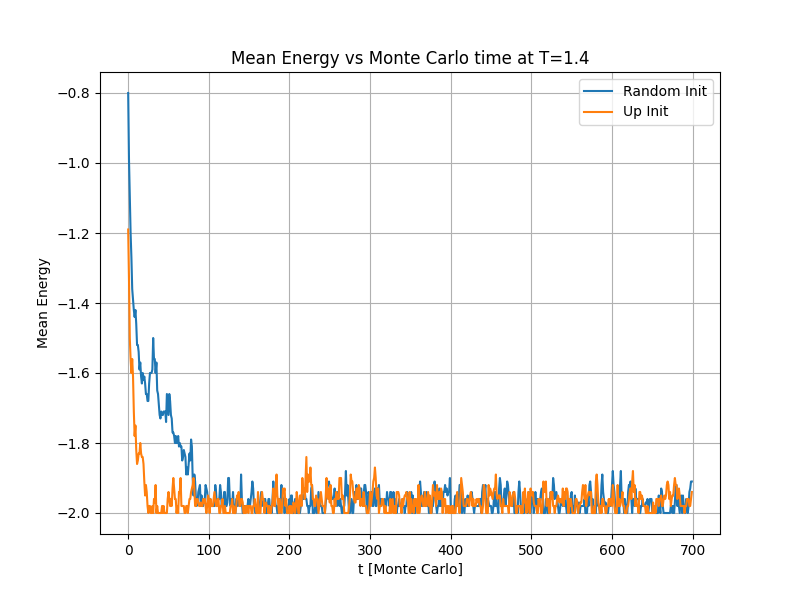
\includegraphics[width=\textwidth]{Mean Energy_tMC.png}
        \caption{Energia media}
        \label{fig:mean_energy}
    \end{subfigure}
    \hfill
    \begin{subfigure}{0.48\textwidth}
        \centering
        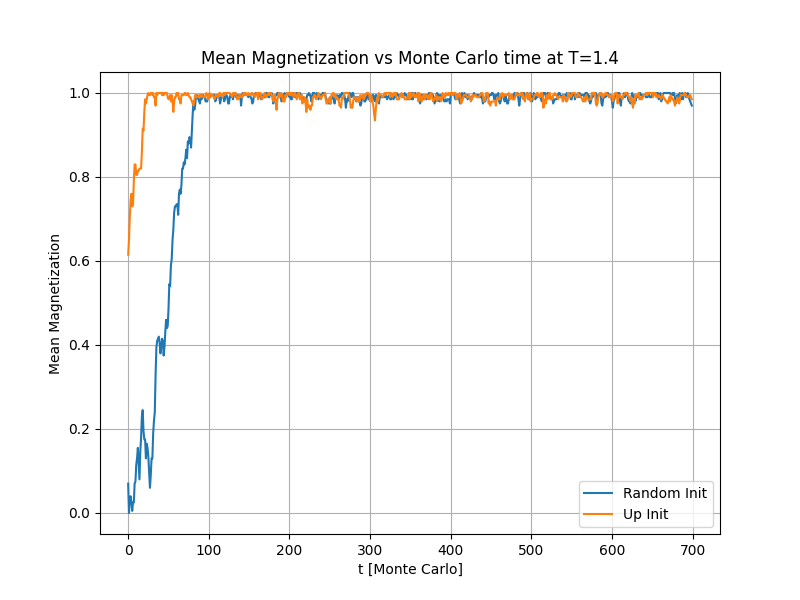
\includegraphics[width=\textwidth]{Mean Magnetization_tMC.png}
        \caption{Magnetizzazione media}
        \label{fig:mean_magnetization}
    \end{subfigure}
    \caption{Termalizzazione del sistema per due diverse configurazioni iniziali.}
    \label{fig:simultation_one}
\end{figure}

La Figura \ref{fig:simulation_two} riporta energia media e magnetizzazione media in funzione della temperatura. 


\begin{figure}[H]
    \centering
    \begin{subfigure}{0.48\textwidth}
        \centering
        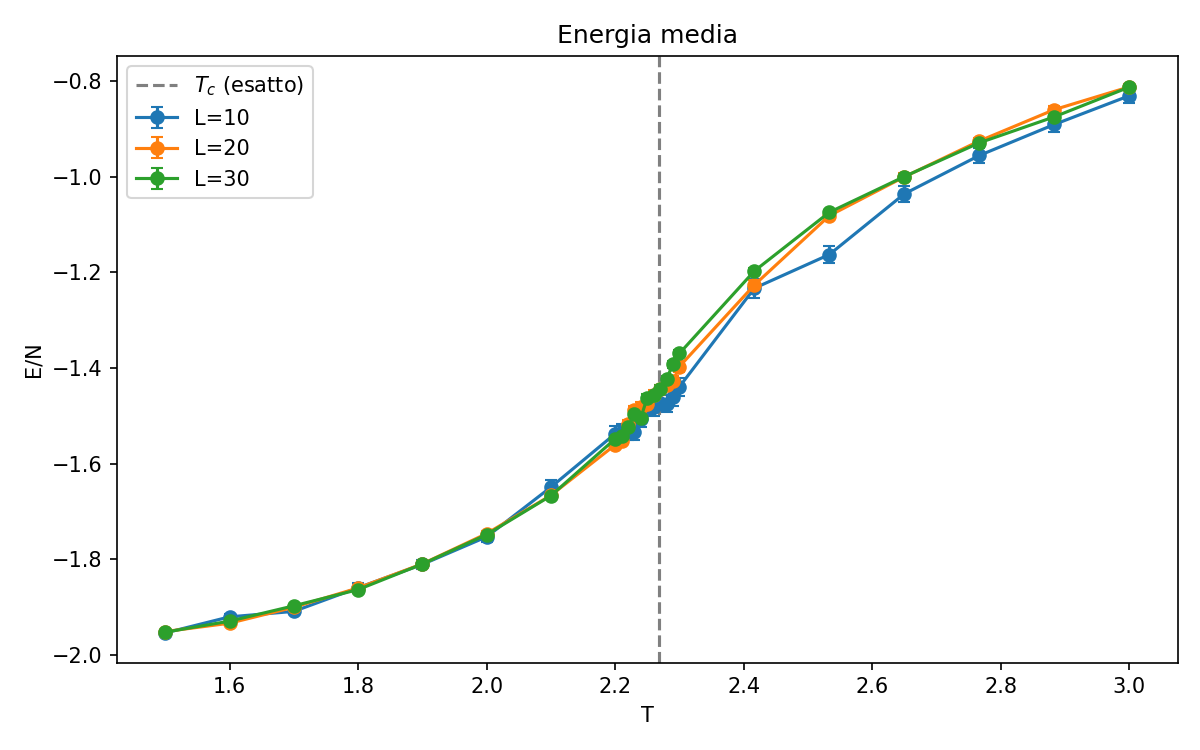
\includegraphics[width=\textwidth]{fss_mean_energies.png}
        \caption{Energia media}
        \label{fig:mean_energy_vs_T}
    \end{subfigure}
    \hfill
    \begin{subfigure}{0.48\textwidth}
        \centering
        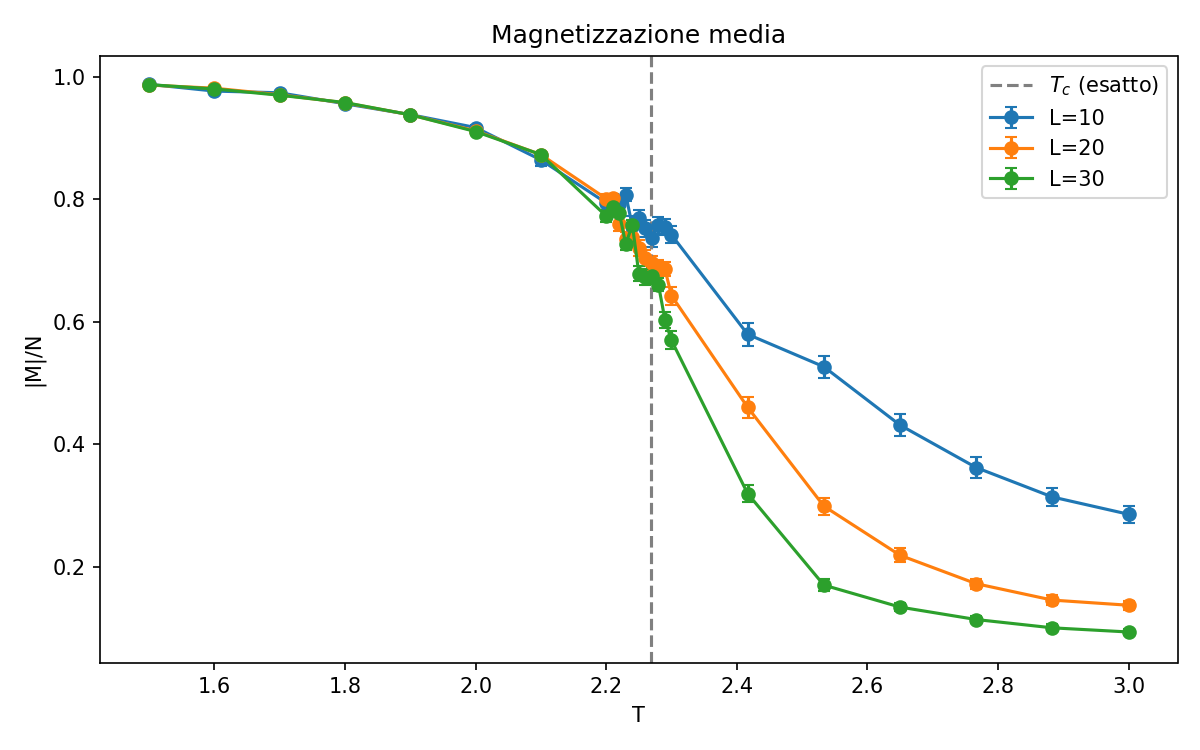
\includegraphics[width=\textwidth]{fss_mean_magnetizations.png}
        \caption{Magnetizzazione media}
        \label{fig:mean_magnetization_vs_T}
    \end{subfigure}
    \caption{Energia media e magnetizzazione media in funzione della temperatura.}
    \label{fig:simulation_two}
\end{figure}

L’energia varia in modo regolare e continuo, mentre la magnetizzazione mostra un comportamento tipico di una transizione di fase: per basse temperature il sistema presenta ordine ferromagnetico con $\langle |M| \rangle \neq 0$, mentre al di sopra di una temperatura critica $T_c$ la magnetizzazione si annulla nel limite termodinamico.

La Figura \ref{fig:simultation_three} mostra il calore specifico e la suscettibilità. Entrambe le quantità presentano un picco in corrispondenza della temperatura critica. 

Il picco del calore specifico è associato alle fluttuazioni energetiche, mentre quello della suscettibilità è legato alle fluttuazioni della magnetizzazione. L’aumento delle fluttuazioni in prossimità di $T_c$ è una firma della criticità del sistema.

Nel limite di sistema infinito, tali grandezze presentano un comportamento non analitico; nel sistema finito simulato si osserva invece un massimo arrotondato, la cui altezza cresce all’aumentare di $L$.

\begin{figure}[H]
    \centering
    \begin{subfigure}{0.48\textwidth}
        \centering
        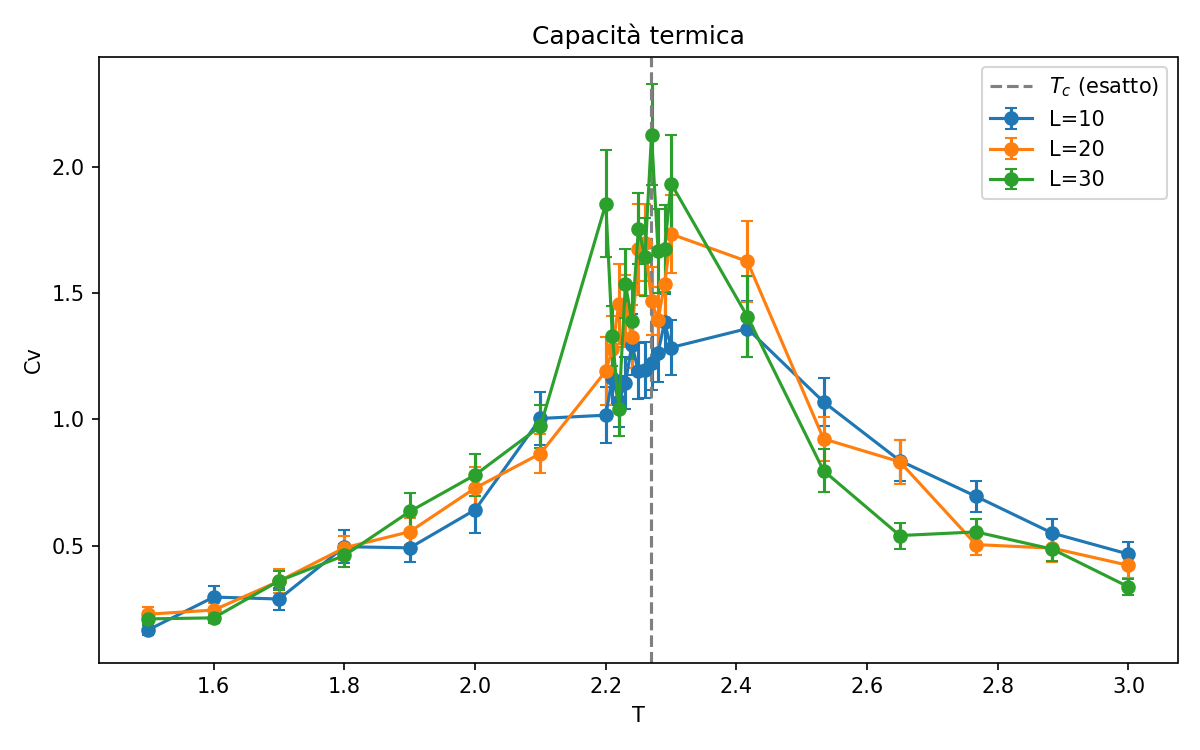
\includegraphics[width=\textwidth]{fss_heat_capacity.png}
        \caption{Calore specifico}
        \label{fig:heat_capacity}
    \end{subfigure}
    \hfill
    \begin{subfigure}{0.48\textwidth}
        \centering
        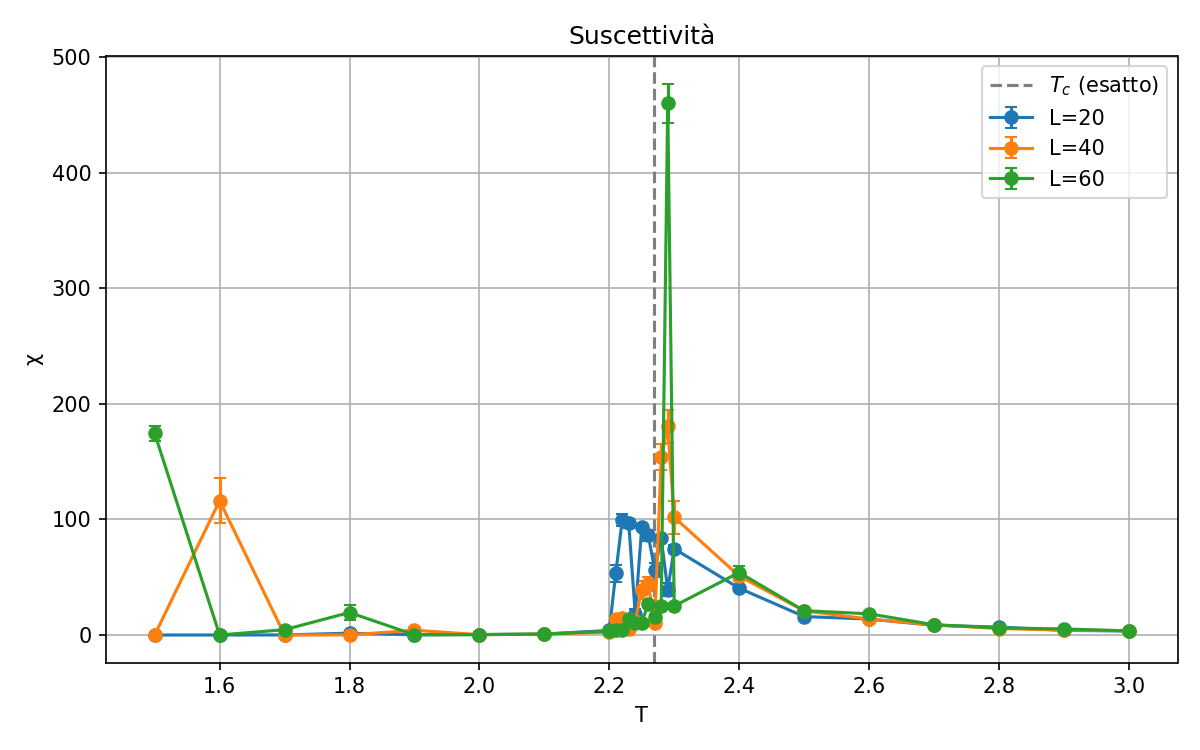
\includegraphics[width=\textwidth]{fss_susceptibility.png}
        \caption{Suscettibilità}
        \label{fig:susceptibility}
    \end{subfigure}
    \caption{Capacità termica e suscettibilità in funzione della temperatura.}
    \label{fig:simultation_three}
\end{figure}

\subsection{Stima della temperatura critica e finite-size scaling}

Per stimare la temperatura critica $T_c$ del sistema, si è utilizzato il metodo di finite-size scaling. Esso si basa sull’osservazione che, 
in un sistema finito, le grandezze fisiche non presentano discontinuità ma mostrano un comportamento arrotondato, 
con picchi che si spostano e si accentuano al crescere della dimensione del sistema.

L'equazione di finite-size scaling per la suscettibilità $\chi$ è data da:
\begin{equation}
    T_c^{*}(L) = T_c + a L^{-1/\nu}
\end{equation}
dove $T_c^{*}(L)$ è la temperatura alla quale si osserva il picco della suscettibilità per un sistema di dimensione $L$, $T_c$ è la temperatura critica nel limite termodinamico, $a$ è una costante e $\nu$ è l'esponente critico associato alla lunghezza di correlazione.
Utilizzando i dati ottenuti dalle simulazioni per diverse dimensioni del sistema, è stato possibile effettuare un fit lineare di $T_c^{*}(L)$ in funzione di $L^{-1/\nu}$, con $\nu = 1$ per il modello di Ising bidimensionale.

\begin{figure}[H]
    \centering
    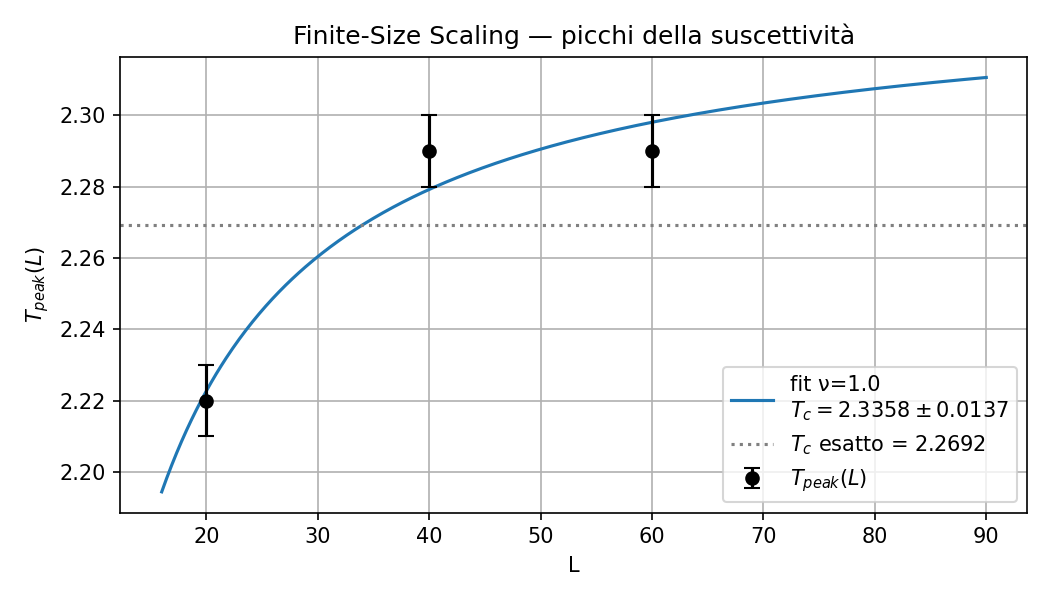
\includegraphics[width=0.6\textwidth]{fss_Tc.png}
    \caption{Stima della temperatura critica $T_c$ mediante finite-size scaling.}
    \label{fig:Tc_fss}
\end{figure}

\section{PCA: Principal Component Analysis}
\subsection{Definizione}

\section{Conclusioni}
In questo lavoro è stato studiato il modello di Ising bidimensionale attraverso tre approcci distinti, mostrando 
come i tre approcci si rivelino complementari e sinergici nello studio del modello: 
la teoria di campo medio offre intuizione analitica, le simulazioni MC permettono di quantificare con precisione 
le osservabili termodinamiche, 
e la PCA dimostra il potenziale degli strumenti di data science nell'esplorazione di sistemi fisici complessi.

La teoria di campo medio ha fornito una descrizione analitica della transizione, 
stimando una temperatura critica $T_C^{MF}= \frac{4J}{k_b}$, che sovrastima il valore esatto di Onsager$ T_C \approx 2.269 \frac{J}{k_b}$.
Tale discrepanza è dovuta al fatto che sono state trascurate le fluttuazioni locali degli spin, che risultano particolarmente rilevanti in prossimità della transizione di fase.

Le simulazioni Monte Carlo con algoritmo di Metropolis hanno consentito 
di riprodurre numericamente le principali grandezze termodinamiche del sistema. I risultati ottenuti
sono in buon accordo con la soluzione esatta: le stime della temperatura critica, ricavate 
dal picco della suscettività e del calore specifico sono compatibili con il valore esatto calcolato da Onsager entro 
gli errori stimati.

Infine, l'applicazione della PCA alle configurazioni generate con 
Monte Carlo ha mostrato come tecniche di apprendimento 
automatico non supervisionato siano in grado di identificare 
automaticamente il parametro d'ordine del sistema e la transizione di fase, 
senza alcuna conoscenza a priori della fisica sottostante. La prima componente principale
risulta correlata quasi perfettamente con la magnetizzazione ($r \approx \ 1$), mentre 
la seconda componente riflette il comportamento della suscettività ($ r \approx \ 0.7).


\section{Appendice}

\subsection{Espansione della suscettività magnetica}\label{appendice:calcolo_suscettivita}

\bibliographystyle{unsrt}
\bibliography{bibliografia}

\end{document}